%
% Einstein Platform User�s Manual (2006.6)
%
% Code source LaTeX2e.
%
% Requiert un certain nombre de paquets (fournis avec la distribution de 
% i-Packages et sans doute la plupart des distributions):
% - palatino
% - hyperref
%
\documentclass[a4paper, english, 11pt]{article}
\usepackage{graphicx}
\usepackage{amssymb}
\usepackage{palatino}
\usepackage[applemac]{inputenc}
\usepackage[english]{babel}
\usepackage[T1]{fontenc}
\usepackage[top=2cm,bottom=2cm,left=1.5cm,right=1.5cm]{geometry}
\usepackage[
	bookmarksopen=true,
	pdfstartview=,
	pdftitle=Einstein\ Platform\ User�s\ Manual,
	pdfauthor=Paul\ Guyot,
	pdfborder=false]{hyperref}
\title{\Huge Einstein Platform\\
User�s Manual\\
�\\
\small{For Einstein Platform 2006.6}}
\begin{document}
% Param�tres pour le document:
% ajustage de l'espace entre les caract�res pour la justification
\setlength{\emergencystretch}{12em}
% macro pour ins�rer une URL
\def\url#1{\href{#1}{\underline {\tt {#1}}}}
\maketitle
%
\newpage
\tableofcontents
\newpage
% espace entre les paragraphes
\parskip = 0.2in
\parindent = 0.0in
\pagestyle{myheadings}
\markright{Einstein Platform User�s Manual}
\section{Introduction}
Einstein Platform is a way to transform a computer in a next-generation Newton N2
(MP2x00, eMate 300).

Einstein is a project to unchain NewtonOS from existing hardware. More information can be found on the Einstein Project home page:
\url{http://kallisys.com/newton/einstein/}

\newpage
\section{Requirements}

Einstein Platform runs on the following machines~:
\begin{itemize}
\item Arm-linux PDAs with X11, libc 2.3.3 with soft FPU and enough memory, such as the Zaurus SL-5500 with OpenZaurus.
\item A Nokia 770.
\item A Mac with a G4 or higher, running 10.3.9 or higher.
\item A MacIntel running 10.4.6 or higher.
\end{itemize}

Einstein Platform requires 40 MB of storage.

\begin{itemize}
\item Einstein Platform requires an MP2x00 US, an MP2x00 D or an eMate 300 ROM image.
\end{itemize}

Instructions about how to extract the ROM are available in the next section.

PLEASE DO NOT ASK ME FOR A ROM FILE. I will not provide you with any.
NewtonOS ROM is copyright by Apple Computer, Inc and licensors.

\newpage
\section{Extraction of the ROM from your Newton}

Two methods are available: via a serial line or via TCP/IP (i.e. via an Ethernet access).

\subsection{Hammer/Newtsbug (serial line)}

Using a low-level debugger such as Hammer or Newtsbug, you can make a dump of the memory. This is slow and works over the serial line.

\underline{Requirements:}
\begin{itemize}
\item A computer running in Classic or MacOS < X
\item Hammer or Newtsbug (they can be found on UNNA, \url{http://www.unna.org/})
\item A serial connection between your Newton and the Mac:
\begin{itemize}
\item a built-in serial port for computers booting in MacOS < X
\item or a USB to Serial port adapter compatible with Classic.
\end{itemize}
\end{itemize}

\underline{Steps:}
\begin{itemize}
\item Install Debugger Connection or Newtsbug Connection package on your Newton.
\item Plug the Newton with the Mac using the serial line.
\item Run Hammer or Newtsbug on the Mac.
\end{itemize}
A standard get file dialog appears: choose the debugging image corresponding to your Newton (Senior CirrusNoDebug image, Senior DCirrusNoDebug image or Newt KNoDebug image for the MP2x00 US, MP2100 or eMate 300 respectively).
\begin{itemize}
\item Tap the Debugger Connection or Newtsbug Connection package on your Newton and choose connect.
\item On the Mac, once the connection is established, choose Save Memory from the File menu.
\item Save memory between 0 and 00800000 (8 MB).
\end{itemize}

Wait.

\subsection{ROM Dumper (TCP/IP)}

ROM Dumper is a faster approach but requires an internet connection between your Mac (or any Unix computer) and your Newton.

\underline{Requirements}
\begin{itemize}
\item A working TCP/IP or Internet connection between your Newton and your Mac.
\end{itemize}

\underline{Steps:}
\begin{itemize}
\item Install provided ROM Dumper package on your Newton.
\item Tap the ROM Dumper icon in the Extras Drawer.
\item Tap start.
\item If your Newton isn�t connected to the Internet yet, choose a connection method. It�s also the time to insert your Ethernet/WiFi card.
\item Note the IP of the Newton (ROM Dumper mentions it).

\begin{center}
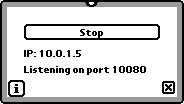
\includegraphics[width=6cm]{ROMDumper.png}\\
\emph{ROM Dumper listening}
\end{center}

\item Launch Einstein Platform (the GUI version).
\item Choose Dump ROM from the Einstein menu.

\begin{center}
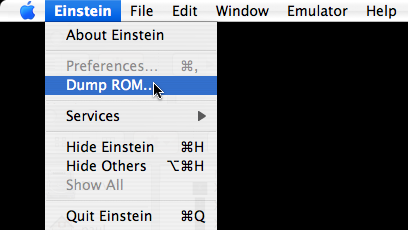
\includegraphics[width=12cm]{DumpROMMenuItem.png}\\
\emph{Dump ROM Menu Item}
\end{center}

\item Type the IP address of your Newton.

\begin{center}
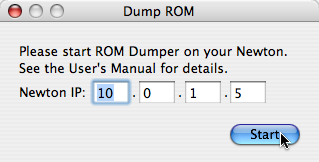
\includegraphics[width=8cm]{DumpROMPanel.png}\\
\emph{Dump ROM Panel}
\end{center}

\item Click start.
\item Mention where to save the Newton ROM. Be careful not to erase previously dumped ROM file if you are dumping the ROM of several different Newton models.
\item Wait (a little bit).
\end{itemize}

The platform will be configured to use the newly dumped ROM.

Alternatively, you can use nc(1) command line tool.

\newpage
\section{Einstein on MacOS X}

Just copy the GUI application to your hard drive and double click it. The first time, it will ask you to tell it where the ROM image is.

You can run Einstein Platform full screen. To exit Einstein, go to the Extras Drawer, tap the [i] button and then choose Quit Einstein.

On MacOS X, Einstein application is scriptable. You can install packages or evaluate NewtonScript code within Einstein Platform using AppleScript.

\subsection{Using the CLI flavor on MacOS X}

On desktop computers, the CLI flavor should mainly be used to access the log and/or the monitor mode. It is therefore intended for developers.

\begin{itemize}
\item Name the ROM dump either:
717006 (MP2x00 US)
737041 (MP2100 D)
747129 (eMate 300)

\item Put the file in the data directory, next to Einstein.rex file (Einstein.rex is
the ROM Extension for Einstein Platform, it includes Einstein drivers and
Frank Gruendel's NewtTest program).

\item Then, in the Einstein directory, launch Einstein with:
\verb|$ ./einstein --machine=XXXX data|
\end{itemize}

where XXXX should be either:
717006 (for a MP2x00 US)
737041 (for a MP2100 D)
747129 (for an eMate 300)

\subsection{Options}
\verb|./einstein --help| will print some help about the options. The options are summarized below:

\verb|--audio| or |-a|\\
Select the audio driver (null, portaudio or coreaudio). \verb|--audio=null| will disable sound. \verb|--audio=portaudio| will choose portaudio sound driver. Default is coreaudio.

\verb|--width|\\
Set the width of the screen (in portrait mode). Default is 320.

\verb|--height|\\
Set the height of the screen (in portrait mode). Default is 480.

\verb|--log| or \verb|-l|\\
Set the log file. Default is to not log. This option is incompatible with --monitor.

\verb|--machine| or \verb|-m|\\
Set the machine. Choose 717006 for a MP2x00 US, 737041 for a MP2100D or 747129 for an eMate 300. \verb|--machine| option can be omitted with a 717006 ROM file.

\verb|--monitor|\\
Run in monitor mode.

\verb|--ram|\\
Set the RAM size in 64 KB increment. 1 will mean 64 KB of RAM. 64 is the default setting (4 MB). The maximum is 255 (nearly 16 MB).

\newpage
\section{Einstein on arm-linux (with SoftFPU) PDAs}

\subsection{Quickstart on the Zaurus}

I used a Zaurus SL-5500 (thanks Sylvain) with OpenZaurus (http://www.openzaurus.org/) 3.5.4-rc
ROM and the following packages:

\begin{itemize}
\item \verb|libstdc++6_3.4.3-r10_arm.ipk|
\item \verb|libts-0.0-0_0.0cvs20050403-r18_arm.ipk|
\item \verb|libx11-6_6.2.1-r2_arm.ipk|
\item \verb|libxau0_0.1.1-r1_arm.ipk|
\item \verb|libxcalibrate0_0.0cvs20050403-r0_arm.ipk|
\item \verb|libxdmcp0_0.1.3-r1_arm.ipk|
\item \verb|libxext6_0.0cvs20050222-r1_arm.ipk|
\item \verb|libxfont1_1.4.2-r2_arm.ipk|
\item \verb|libxft2_2.1.6-r1_arm.ipk|
\item \verb|libxrandr2_1.0.2-r1_arm.ipk|
\item \verb|libxrender1_0.8.4-r1_arm.ipk|
\item \verb|tslib-conf_0.0cvs20050403-r18_collie.ipk|
\item \verb|ttf-bitstream-vera_1.10-r2_all.ipk|
\item \verb|xserver-kdrive-fbdev_20050207-r0_arm.ipk|
\item \verb|xtscal_0.6.3-r0_arm.ipk|
\end{itemize}

Any more recent version of OpenZaurus and these packages should do it.

I first installed the Bootstrap Image with the zImage-64-0 to have enough RAM for Einstein Platform. Then, I copied all these packages to a CF card and I installed them all at once with the ipkg command line tool on the Zaurus (with something like \verb|ipkg install /mnt/cf/*.ipk|).

I fixed the date with \verb|date 053112002006|.

Then, I copied the three elements from the release archive as well as the 710006 ROM image to the root of the CF card. And I launched the script with:
\verb|/mnt/cf/start-einstein.sh|

\subsection{More details for other PDAs}

I haven't tested Einstein Platform on other arm-linux PDAs. Please note that Einstein Platform requires libc 2.3.3 and quite a large amount of RAM. Most PDAs do not provide enough RAM for third party application unless you enter some developer mode or install a bootstrap image.

\begin{itemize}
\item Name the ROM dump either:
717006 (MP2x00 US)
737041 (MP2100 D)
747129 (eMate 300)

\item Put the file on the compact flash, next to Einstein.rex file.

\item Run the X server. Xfbdev on the Zaurus needs to be run at 270 degrees:
\verb|Xfbdev -screen 320x240@270 -dpi 100 &|

\item Run Einstein Platform with:\\
\verb|/mnt/cf/einstein --machine=XXXX --width=YYYY --height=ZZZZ /mnt/cf|
\end{itemize}

where XXXX should be either:
717006 (for a MP2x00 US)
737041 (for a MP2100 D)
747129 (for an eMate 300)

and YYYY and ZZZZ should be set properly.

\subsection{Options}

\verb|./einstein --help| will print some help about the options. The options are summarized below:

\verb|--width|\\
Set the width of the screen (in portrait mode). Default is 320.

\verb|--height|\\
Set the height of the screen (in portrait mode). Default is 480.

\verb|--log| or \verb|-l|\\
Set the log file. Default is to not log. This option is incompatible with --monitor.

\verb|--machine| or \verb|-m|\\
Set the machine. Choose 717006 for a MP2x00 US, 737041 for a MP2100D or 747129 for an eMate 300. \verb|--machine| option can be omitted with a 717006 ROM file.

\verb|--monitor|\\
Run in monitor mode.

\verb|--ram|\\
Set the RAM size in 64 KB increment. 1 will mean 64 KB of RAM. 64 is the default setting (4 MB). The maximum is 255 (nearly 16 MB).

\newpage
\section{Einstein on the Nokia 770}

The first step is to enable root mode. Connect the Nokia to a desktop computer and use the flasher developer tool to enable root mode.

\newpage
\section{Developer notes}
\subsection{CLI commands}

The command line interface is intended for developers and hackers.

Using the cli flavor, you will be provided with a prompt. Typing help will provide a small help about the available commands.

\subsection{Monitor mode}

The monitor mode uses a disassembler from the NetBSD project (the kernel disassembler for the arm32 port). You start in monitor mode by specifying the --monitor option to the command line program.

The monitor mode can be considered as an enhanced low-level debugger. The help command displays a short help for the available commands.

One of the main advantage of the monitor is that you can set breakpoints. You can also halt the emulator by calling the |Einstein:BreakInMonitor| global function (it doesn�t take any parameter).

The following breakpoints are enabled by default:
\begin{itemize}
\item NewtonOS UND instructions to pass strings to the debugger (typically followed by a reboot). They are executed (i.e. the Newton will reboot), but the Newton is halted and the string is printed to the monitor.
\item Some violations that shouldn't happen.
\end{itemize}

You cannot use \verb|--log| option with \verb|--monitor| because in monitor mode, the log is always enabled. You can save the log to a file (it scrolls on the monitor screen).

The monitor mode uses a file with symbols. This file should be named after the ROM file, e.g. 717006.symbols. The syntax is:

\verb|address <tab> symbol <tab> comment|

Addresses should be sorted.

This file is very easy to generate from the debugger images that are used with
Hammer and Newtsbug. Use Newton C++ Tools DumpAIF program with the -s option to dump the list of symbols. Then you can process all the lines with research and replace or sed or awk at your convenience. The symbols can be unmangled with Unmangle tool coming with MPW.

\subsection{Logging}

Quite a large amount of log lines are generated by Einstein. These are used during the development of Einstein emulator. It also helps to understand what�s going on.

Starting with UP2 release, you can generate log lines from NewtonScript calling the |Einstein:Log|�global function.

E.g.:
\begin{verbatim}
|Einstein:Log|("Hello World")
\end{verbatim}

will display \texttt{Hello World} in the log. If log is disabled, the string will be output on stdout.

Please note that your string is converted to ISO-8859-1 before being printed, so non latin characters will not be printed properly in the log.

\newpage
\section{Relativity Developer Guide}

\subsection{Introduction}

Relativity is a new technology embedded into Einstein to allow packages for Einstein to take advantage of host APIs.

Relativity can only be used through NewtonScript for the moment. To use relativity, you need to call \verb|OpenNativeLibrary| NewtonScript function to open a library from the host system.

\noindent \verb|OpenNativeLibrary(|\textit{libraryName}\verb|)|

\noindent \textit{libraryName} is a string representing the name of the library to open. Valid names include \verb|"libc"| or \verb|"libGL"|.

This function returns a library object and throws an exception if an error occurs (for example if the library cannot be found).

\noindent \textit{libraryObject}\verb|:GetFunction(|\textit{functionSpecs}\verb|)|

\textit{functionSpecs} is a frame describing the function to import. This frame has three required slots~:
\begin{itemize}
\item \verb|name| the name of the function.
\item \verb|args| an array with the types of the arguments, from left to right. The types are symbols (see below).
\item \verb|result| the type of the result (see below).
\end{itemize}

This function returns a NewtonScript function you can call.

The types can be the following:
\begin{itemize}
\item \verb|'uint8| unsigned integer, 8 bits
\item \verb|'sint8| signed integer, 8 bits
\item \verb|'uint16| unsigned integer, 16 bits
\item \verb|'sint16| signed integer, 16 bits
\item \verb|'uint32| unsigned integer, 32 bits
\item \verb|'sint32| signed integer, 32 bits
\item \verb|'uint64| unsigned integer, 64 bits (unimplemented yet)
\item \verb|'sint64| signed integer, 64 bits (unimplemented yet)
\item \verb|'float| single precision float number (unimplemented yet)
\item \verb|'double| double precision float number (unimplemented yet)
\item \verb|'longdouble| long double precision float number (unimplemented yet)
\item \verb|'string| string (\verb|const char*|)
\item \verb|'iostring| string for output or input/output (\verb|char*|)
\item \verb|'binary| data (\verb|const void*|)
\item \verb|'iobinary| data for output or input/output (\verb|void*|)
\item \verb|'pointer| any pointer on data.
\end{itemize}

Some types are illegal for return or argument types (for example, you cannot use \verb|iostring| for the return type, use \verb|string| instead).

Then, you can call the function naturally by providing Newton data. The result is returned in the form of Newton data.

Once you are done, you can close the library with the \verb|:Close()| method.

\noindent \textit{libraryObject}\verb|:Close()|

Close the library. The library object should no longer be used afterwards.

\subsection{Sample code}

In this section, we will describe how to call a simple function, \verb|gethostname| that returns the (network) name of the host.

The manual page of \verb|gethostname| provides the necessary information to call the routine.

\begin{verbatim}
GETHOSTNAME(3)          BSD Library Functions Manual          GETHOSTNAME(3)

NAME
    gethostname, sethostname -- get/set name of current host

LIBRARY
    Standard C Library (libc, -lc)

SYNOPSIS
    #include <unistd.h>

    int
    gethostname(char *name, size_t namelen);
\end{verbatim}

This page shows that \verb|gethostname| is in the \verb|libc| library. It also provides the type of the arguments and of the result. The following code calls the function and returns the result.

\begin{verbatim}
begin
  // Open the native library.
  local libc := OpenNativeLibrary("libc");
  // Define the function.
  local gethostnameFn := libc:GetFunction({
      name: "gethostname",
      args: ['iostring, 'sint32],
      result: 'sint32});
  
  // Allocate a buffer to store the hostname.
  // This buffer is a string of 127 unicode characters (+ null).
  local theBuffer := MakeBinary('string, 256);
  // Call the function.
  local theResult := call gethostnameFn with (theBuffer, 127);

  // Close the library.
  libc:Close();
  
  // Determine the outcome of the call.
  if (theResult = 0) then
    // Success.
    return theBuffer;
  else
    // Failure
    return "gethostname failed";
end;
\end{verbatim}	

\newpage
\section{Known problems}

\begin{itemize}
\item Serial ports are not emulated.
\item PCMCIA cards are not emulated. The sockets aren�t entirely emulated yet.
\item The sound volume is reported to be settable by software but the changes are ignored (except when the sound is off on the Newton).
\item Sound input isn't emulated.
\item An error occurs when trying to install system patches.
\item Keys are not translated properly except on the Mac (the keyboard is useless).
\item Rotation doesn't always work well.
\item It is awfully slow.
\end{itemize}

Please drop me a line (\url{mailto:pguyot@kallisys.net}) if you experience a problem which is not in this list.

\newpage
\section{Changes History}

5/31/06 Einstein Platform 2006.6
\begin{itemize}
\item Features:
\begin{itemize}
\item Initial release of Relativity for Einstein.
\item Accelerated some transfers between Einstein and Host.
\item Included several keyboard mappings.
\item Update of PortAudio (from CVS).
\item Included a new set of icons by Michael Vac�k. The toolbar icons reflect the state of Einstein.
\item Fixed an endianess problem with the Cocoa screen manager on Intel machines.
\item The state is now shown on the screen (instead of just: screen is off).
\item Improved the Cocoa preferences panel.
\item Included AppleScript support to evaluate newton script code and to install packages.
\end{itemize}

\item Bug fixes:
\begin{itemize}
\item Fixed a bad bug in the memory emulation that caused crashes, especially with the JIT page cache.
\item Fixed a bug yielding to an abort when the platform was quitted.
\item Fixed a bug with CoreAudio sound on Intel machine.
\item PortAudio sound driver now reverts samples an little endian targets.
\item The tablet region was incorrectly limited to 1023x1023. It's now set to NewtonOS size (2047x2047).
\end{itemize}
\end{itemize}

1/14/06 Einstein Platform Beta
\begin{itemize}
\item Initial release.
\end{itemize}

\newpage
\section{License}

Einstein Platform is copyright 2005-2006 by Paul Guyot.
It is provided as is, without any warranty of any kind.

Einstein Platform includes portaudio v19 (from CVS).

\begin{verbatim}
/*
 * PortAudio Portable Real-Time Audio Library
 * Latest Version at: http://www.portaudio.com/
 *
 * Copyright (c) 1999-2000 Phil Burk and Ross Bencina
 *
 * Permission is hereby granted, free of charge, to any person obtaining
 * a copy of this software and associated documentation files
 * (the "Software"), to deal in the Software without restriction,
 * including without limitation the rights to use, copy, modify, merge,
 * publish, distribute, sublicense, and/or sell copies of the Software,
 * and to permit persons to whom the Software is furnished to do so,
 * subject to the following conditions:
 *
 * The above copyright notice and this permission notice shall be
 * included in all copies or substantial portions of the Software.
 *
 * Any person wishing to distribute modifications to the Software is
 * requested to send the modifications to the original developer so that
 * they can be incorporated into the canonical version.
 *
 * THE SOFTWARE IS PROVIDED "AS IS", WITHOUT WARRANTY OF ANY KIND,
 * EXPRESS OR IMPLIED, INCLUDING BUT NOT LIMITED TO THE WARRANTIES OF
 * MERCHANTABILITY, FITNESS FOR A PARTICULAR PURPOSE AND NONINFRINGEMENT.
 * IN NO EVENT SHALL THE AUTHORS OR COPYRIGHT HOLDERS BE LIABLE FOR
 * ANY CLAIM, DAMAGES OR OTHER LIABILITY, WHETHER IN AN ACTION OF
 * CONTRACT, TORT OR OTHERWISE, ARISING FROM, OUT OF OR IN CONNECTION
 * WITH THE SOFTWARE OR THE USE OR OTHER DEALINGS IN THE SOFTWARE.
 *
 */
\end{verbatim}

Einstein Platform also includes NetBSD arm disassembler.

\begin{verbatim}
// $NetBSD: disassem.c,v 1.14 2003/03/27 16:58:36 mycroft Exp $
//
// Copyright (c) 1996 Mark Brinicombe.
// Copyright (c) 1996 Brini.
//
// All rights reserved.
//
// Redistribution and use in source and binary forms, with or without
// modification, are permitted provided that the following conditions
// are met:
// 1. Redistributions of source code must retain the above copyright
//    notice, this list of conditions and the following disclaimer.
// 2. Redistributions in binary form must reproduce the above copyright
//    notice, this list of conditions and the following disclaimer in the
//    documentation and/or other materials provided with the distribution.
// 3. All advertising materials mentioning features or use of this software
//    must display the following acknowledgement:
//	This product includes software developed by Brini.
// 4. The name of the company nor the name of the author may be used to
//    endorse or promote products derived from this software without specific
//    prior written permission.
//
// THIS SOFTWARE IS PROVIDED BY BRINI ``AS IS'' AND ANY EXPRESS OR IMPLIED
// WARRANTIES, INCLUDING, BUT NOT LIMITED TO, THE IMPLIED WARRANTIES OF
// MERCHANTABILITY AND FITNESS FOR A PARTICULAR PURPOSE ARE DISCLAIMED.
// IN NO EVENT SHALL BRINI OR CONTRIBUTORS BE LIABLE FOR ANY DIRECT,
// INDIRECT, INCIDENTAL, SPECIAL, EXEMPLARY, OR CONSEQUENTIAL DAMAGES
// (INCLUDING, BUT NOT LIMITED TO, PROCUREMENT OF SUBSTITUTE GOODS OR
// SERVICES; LOSS OF USE, DATA, OR PROFITS; OR BUSINESS INTERRUPTION)
// HOWEVER CAUSED AND ON ANY THEORY OF LIABILITY, WHETHER IN CONTRACT, 
// STRICT LIABILITY, OR TORT (INCLUDING NEGLIGENCE OR OTHERWISE) ARISING IN
// ANY WAY OUT OF THE USE OF THIS SOFTWARE, EVEN IF ADVISED OF THE
// POSSIBILITY OF SUCH DAMAGE.
\end{verbatim}

\end{document}
